\begin{minipage}{0.55\textwidth}
    \begin{figure}[h]
    \centering
    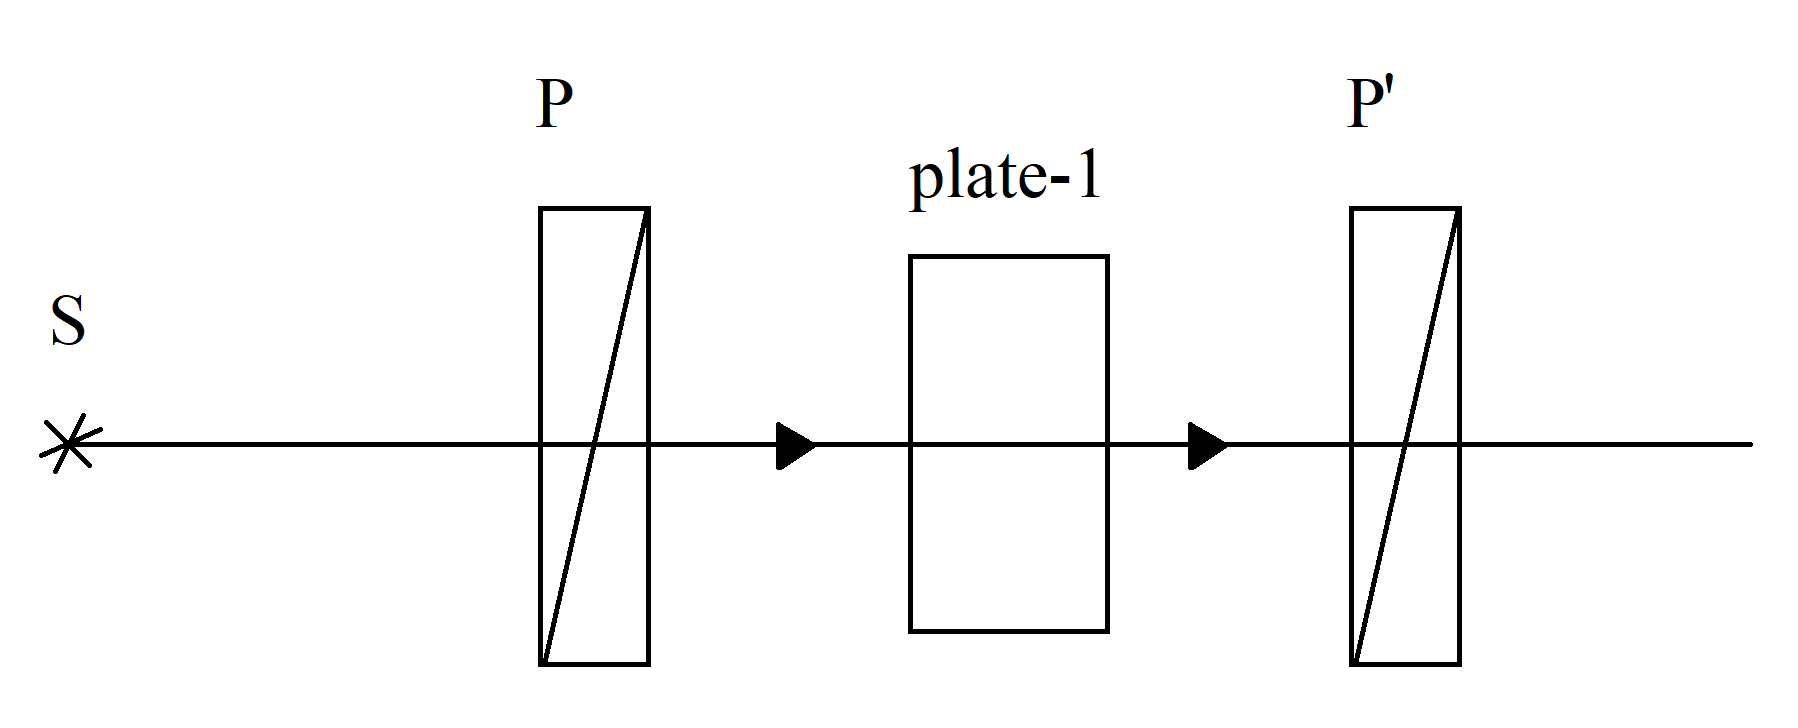
\includegraphics[width=1\textwidth]{images/crystplast.png}
    \caption{We add two crossed polaroids and the double refracting plate between them.}
    %\label{fig:}
\end{figure}
\end{minipage}
\hfill
\begin{minipage}{0.35\textwidth}
    So, when the polarizations match we observe maximum, and otherwise minimum of intensity.
    \begin{align*}
        \text{max} \colon 227^\circ\\
        \text{min} \colon 275^\circ
    \end{align*}
\end{minipage}
